\chapter{Supplementary Diagnostics for Linear and Nonlinear TTM Surrogates}
\label{app:ch4-sampling-support}

This appendix collects distributional diagnostics that support the sampling choices used in Chapter~\ref{ch:regression}. The figures and tables are included as provenance for the linear material-support checks, the nonlinear sampling design, and the staged nonlinear surrogate diagnostics. They are supplementary checks rather than a replacement for the main Chapter~\ref{ch:regression} narrative.

\section{Real-material support for the linear pTTM validation set}

Figure~\ref{fig:app-ch4-linear-material-parameters} summarises the selected real-material thermophysical and optical quantities used to contextualise the linear pTTM validation cases. The figure complements the percentile-support heatmap in Figure~\ref{fig:ch4-material-feature-support} by showing the raw material-level variation behind that support diagnostic.

\begin{figure}[H]
    \centering
    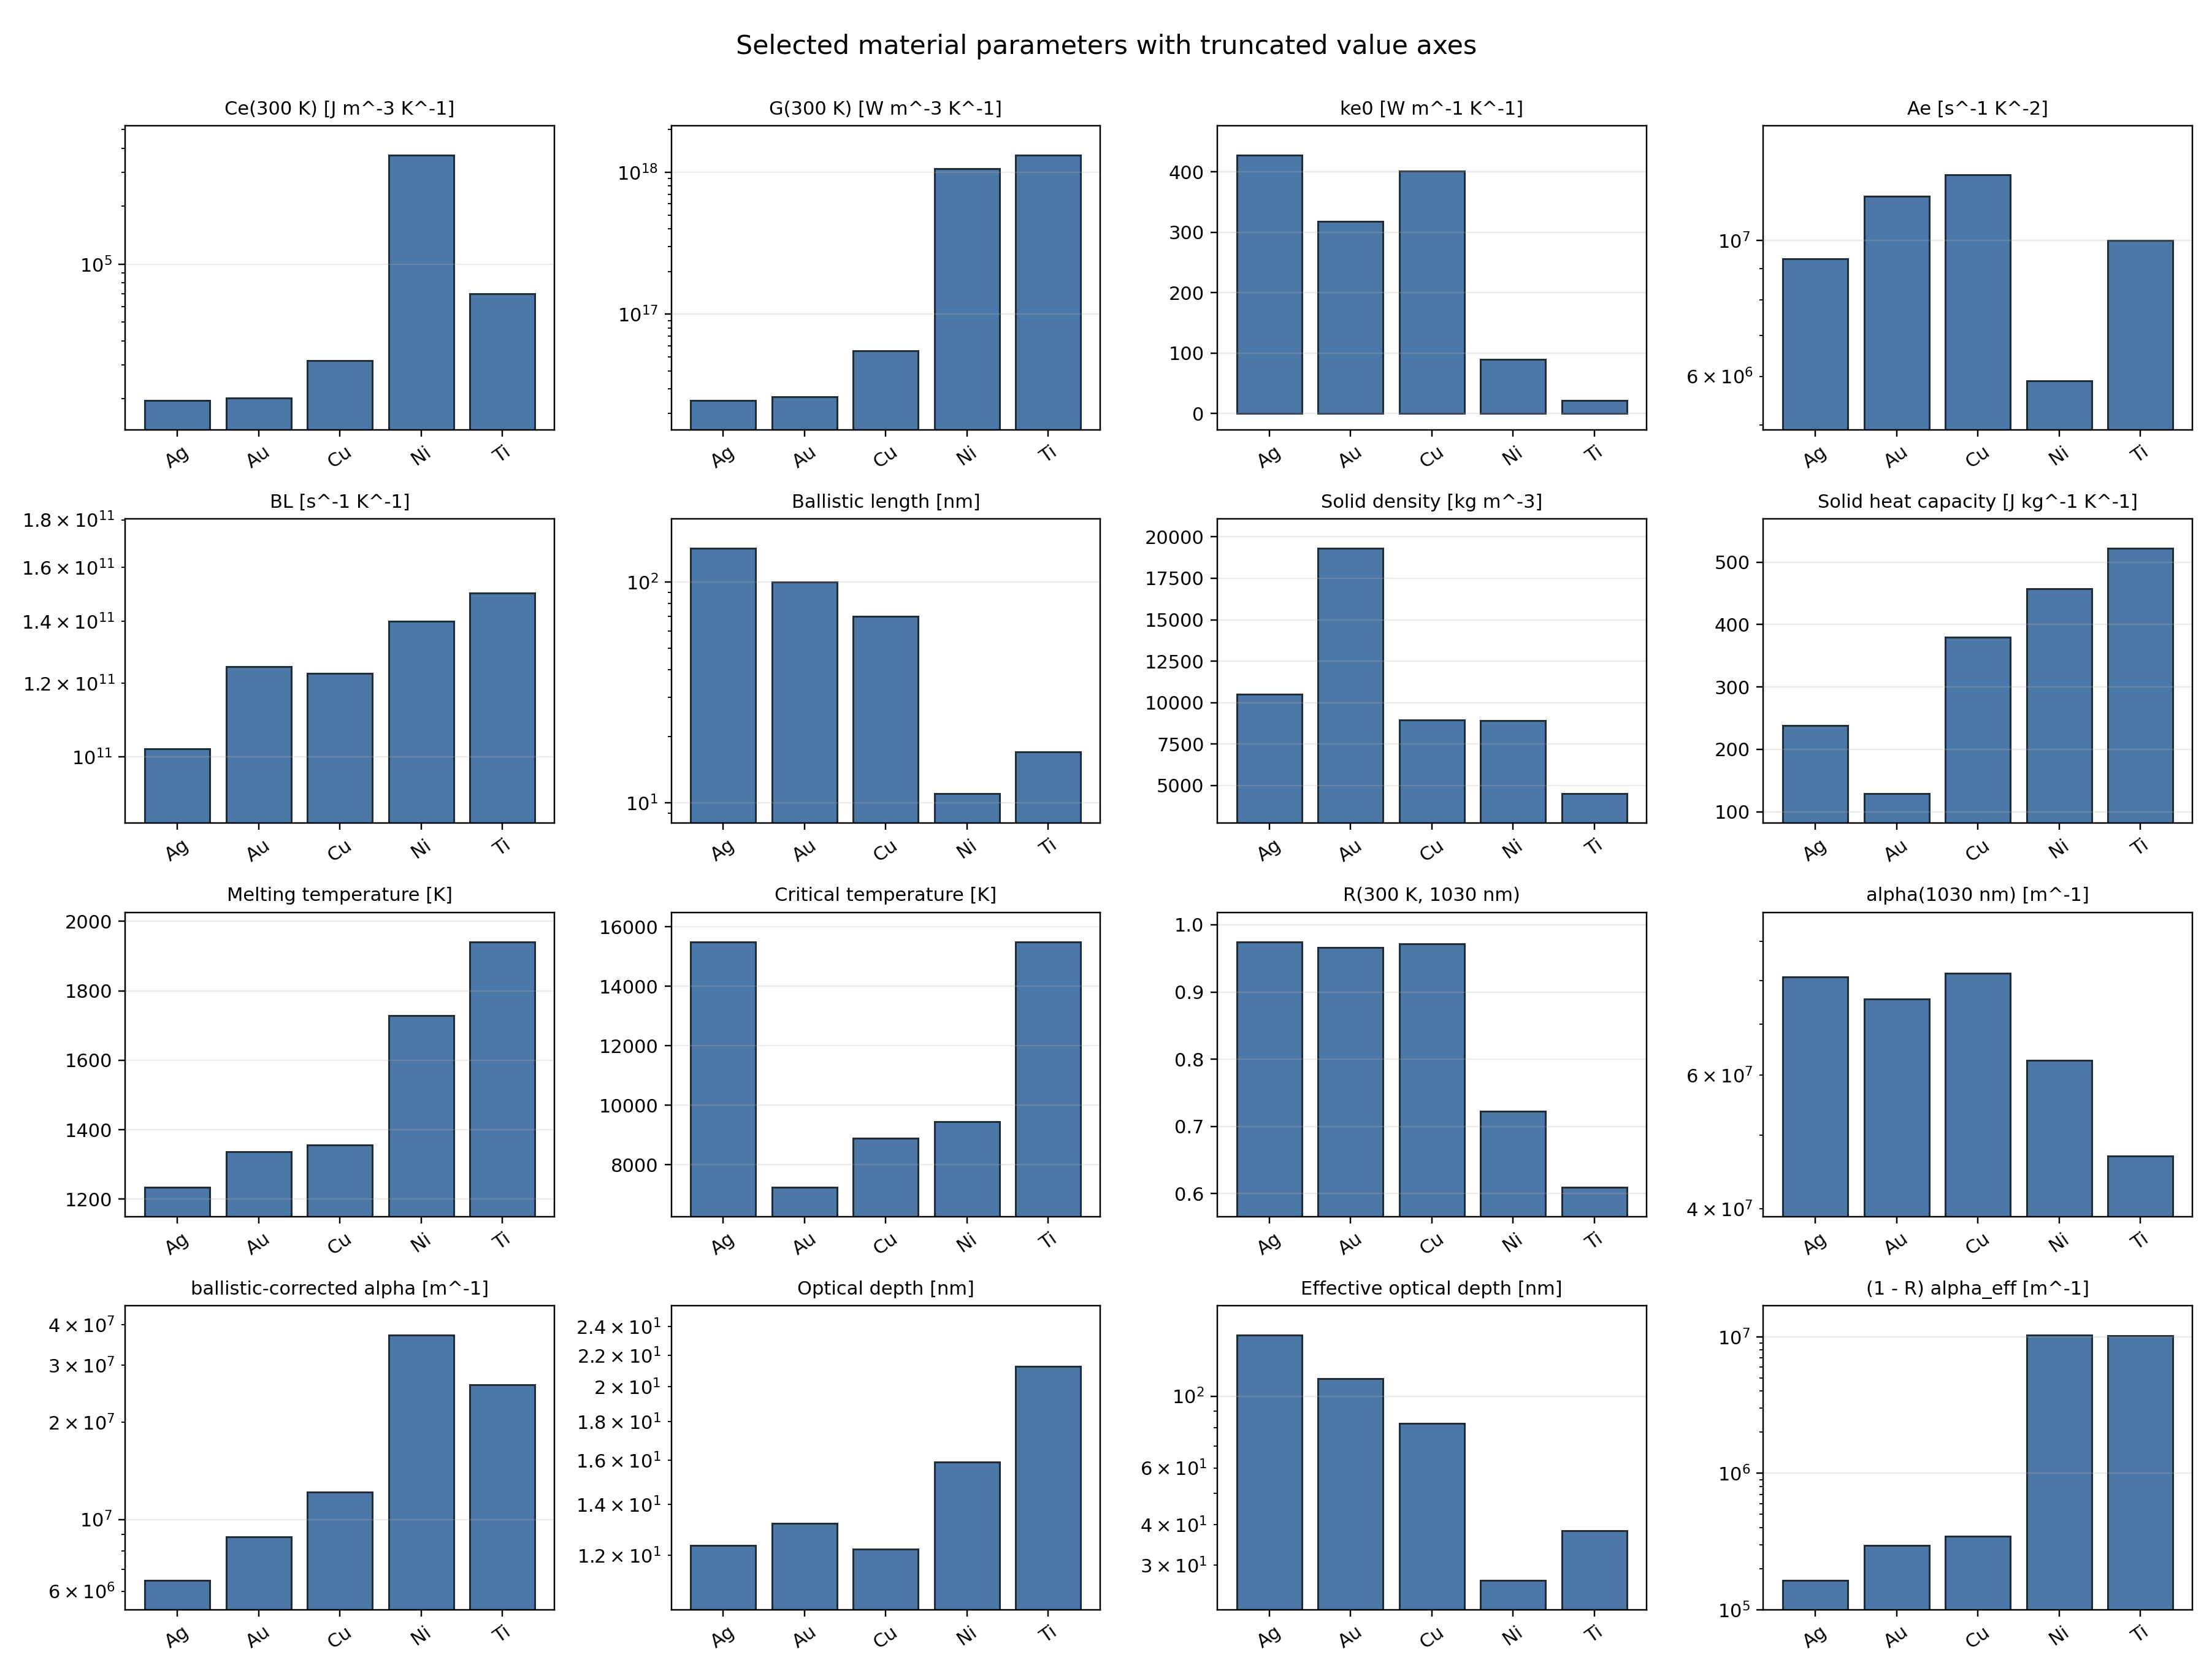
\includegraphics[width=0.96\textwidth]{figures/ch4/linear_ttm/selected_material_physical_parameters_linear.png}
    \caption{Selected real-material physical, thermophysical, and optical parameters for the linear pTTM validation materials. The truncated axes make cross-material variation visible while preserving the role of the figure as support evidence rather than a primary result.}
    \label{fig:app-ch4-linear-material-parameters}
\end{figure}

\section{Real-material Lorentz--Drude descriptor support}

The nonlinear extension in Chapter~\ref{ch:regression} samples optical inputs as Lorentz--Drude descriptors before deriving reflectivity and absorption. Figure~\ref{fig:app-ch4-ld-oscillator-histograms} records the real-material descriptor support used to motivate that choice, including plasma frequency, oscillator strengths, damping factors, and resonance energies.

\begin{figure}[H]
    \centering
    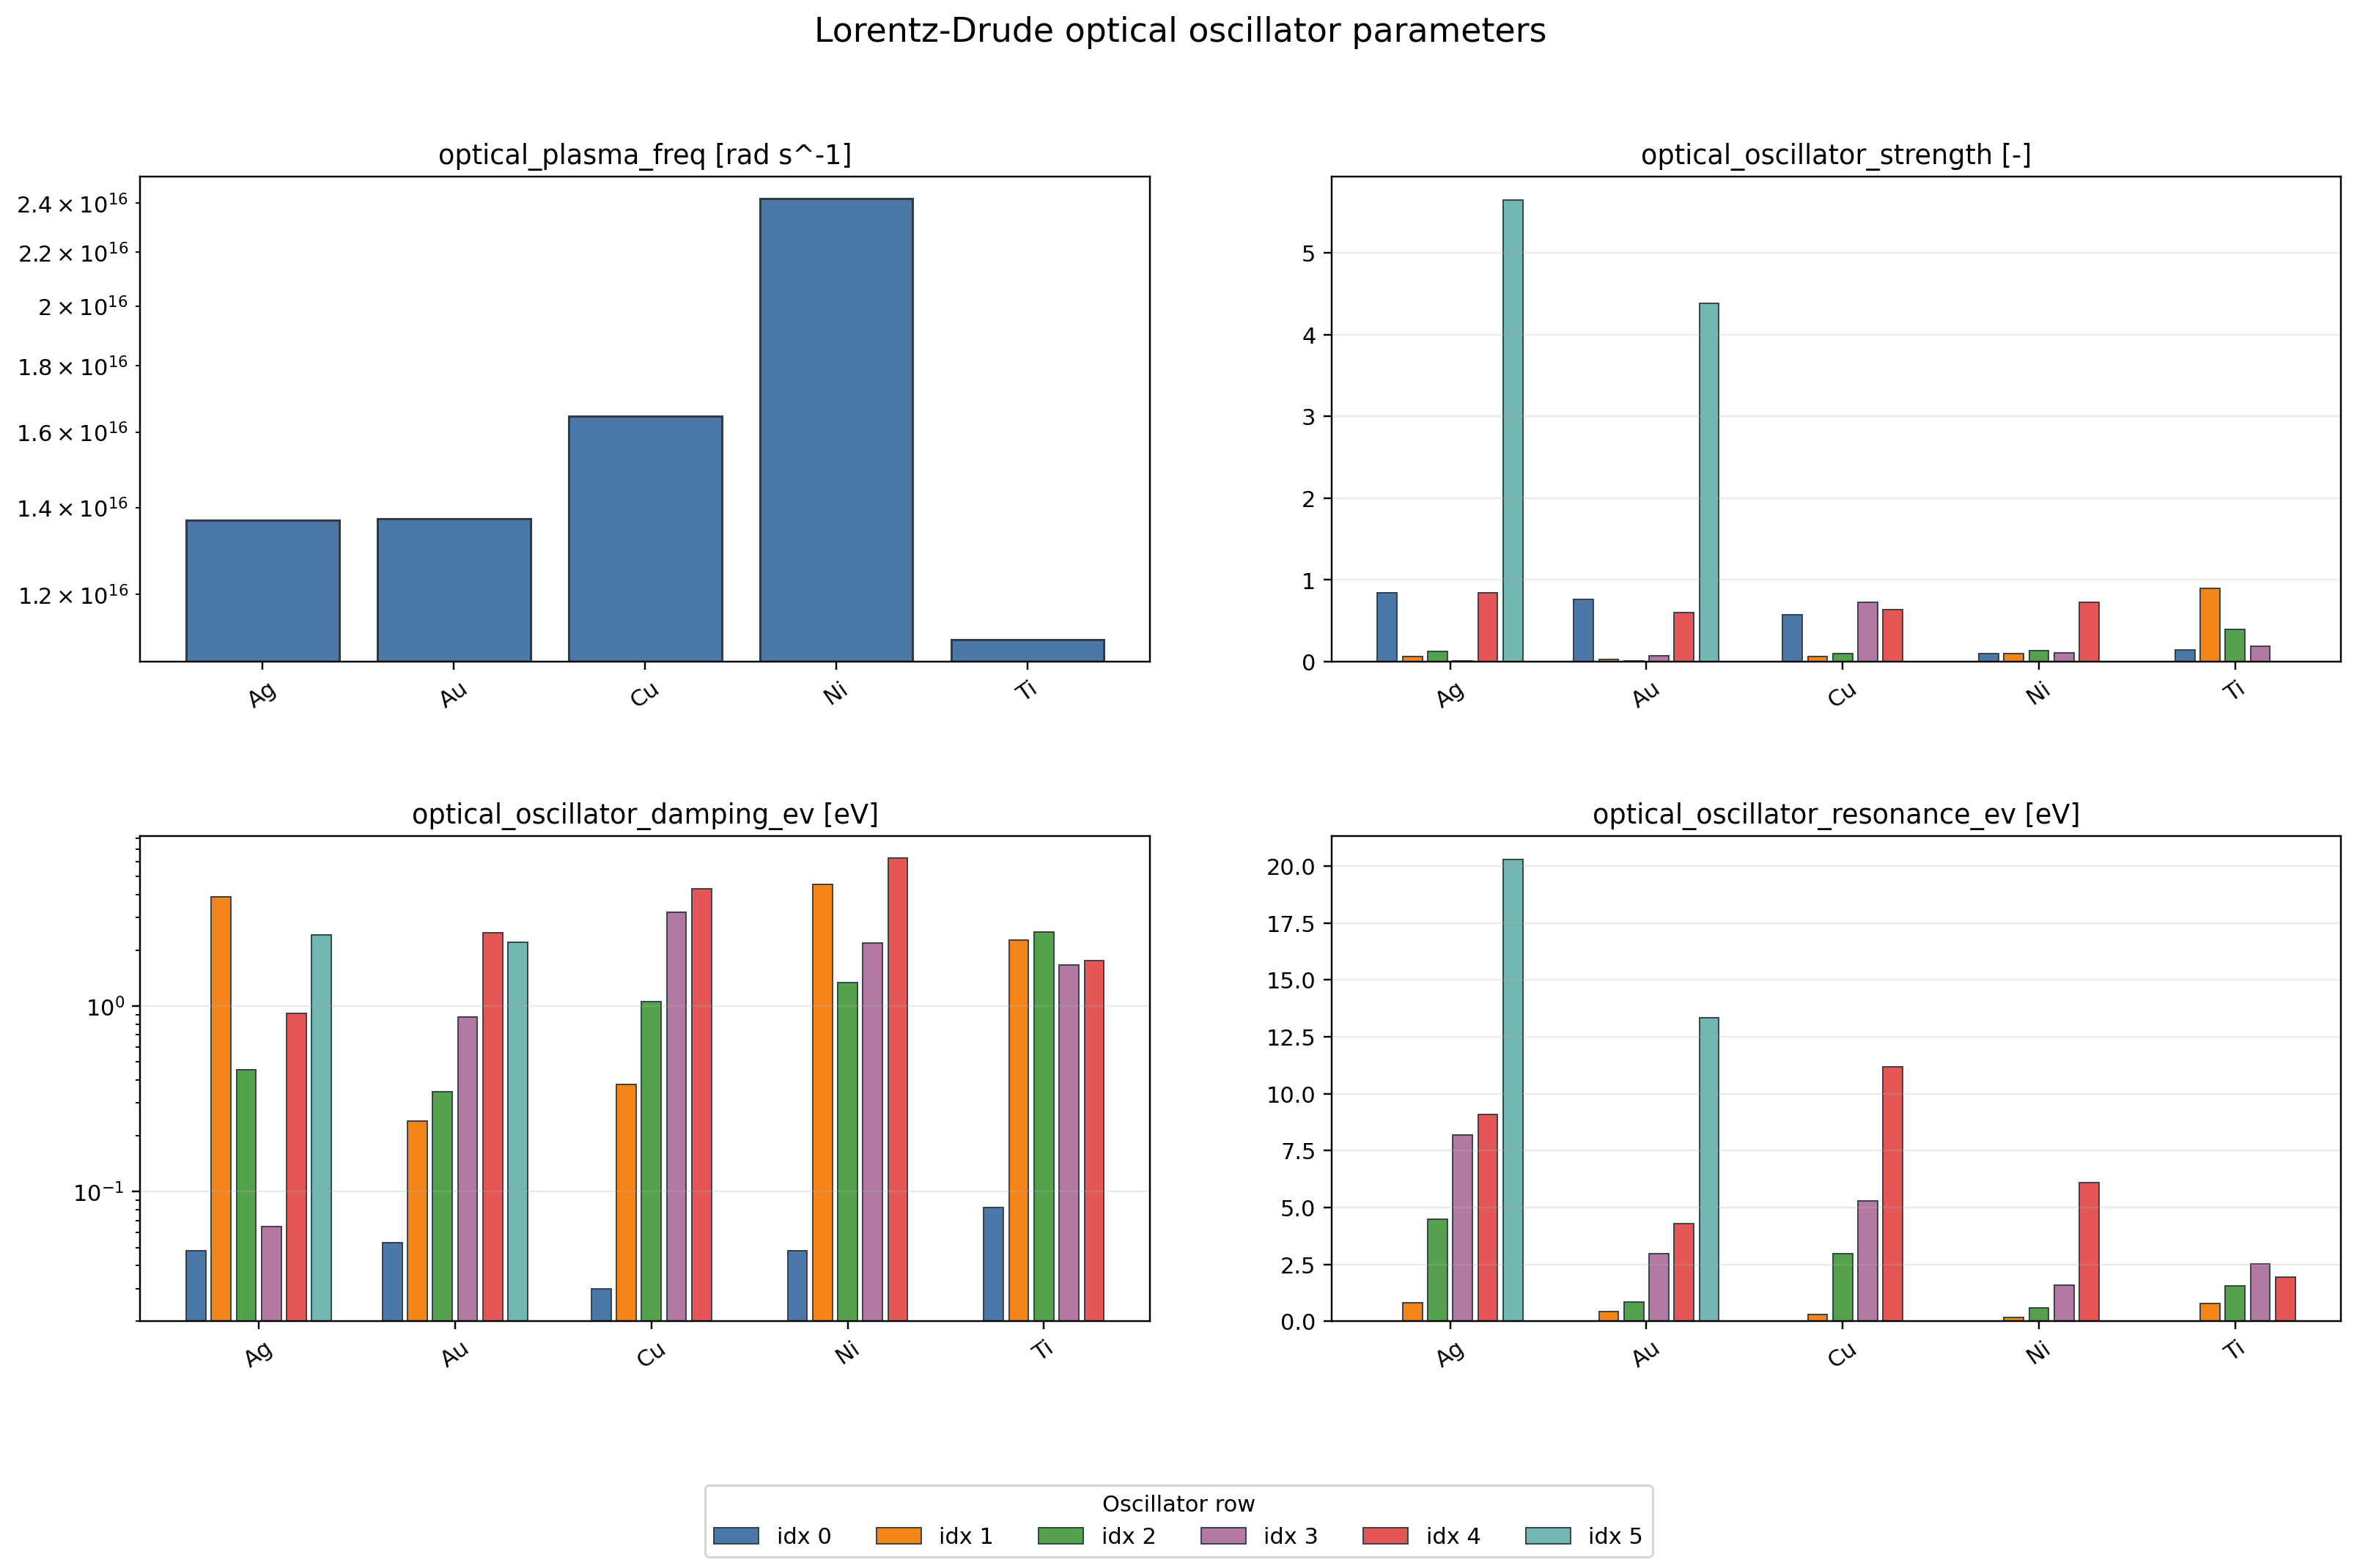
\includegraphics[width=0.96\textwidth]{figures/ch4/nonlinear_ttm/real_material_ld_oscillator_histograms.png}
    \caption{Real-material Lorentz--Drude optical oscillator descriptor distributions used to motivate descriptor-level optical sampling in the nonlinear pTTM extension.}
    \label{fig:app-ch4-ld-oscillator-histograms}
\end{figure}

\section{Synthetic nonlinear sampling diagnostics}

Figures~\ref{fig:app-ch4-nonlinear-sampled-marginals}--\ref{fig:app-ch4-nonlinear-correlation-diagnostic} document the accepted synthetic nonlinear sampling distribution. These diagnostics support the methodology of Chapter~\ref{ch:regression}; they do not report nonlinear model accuracy.

\begin{figure}[H]
    \centering
    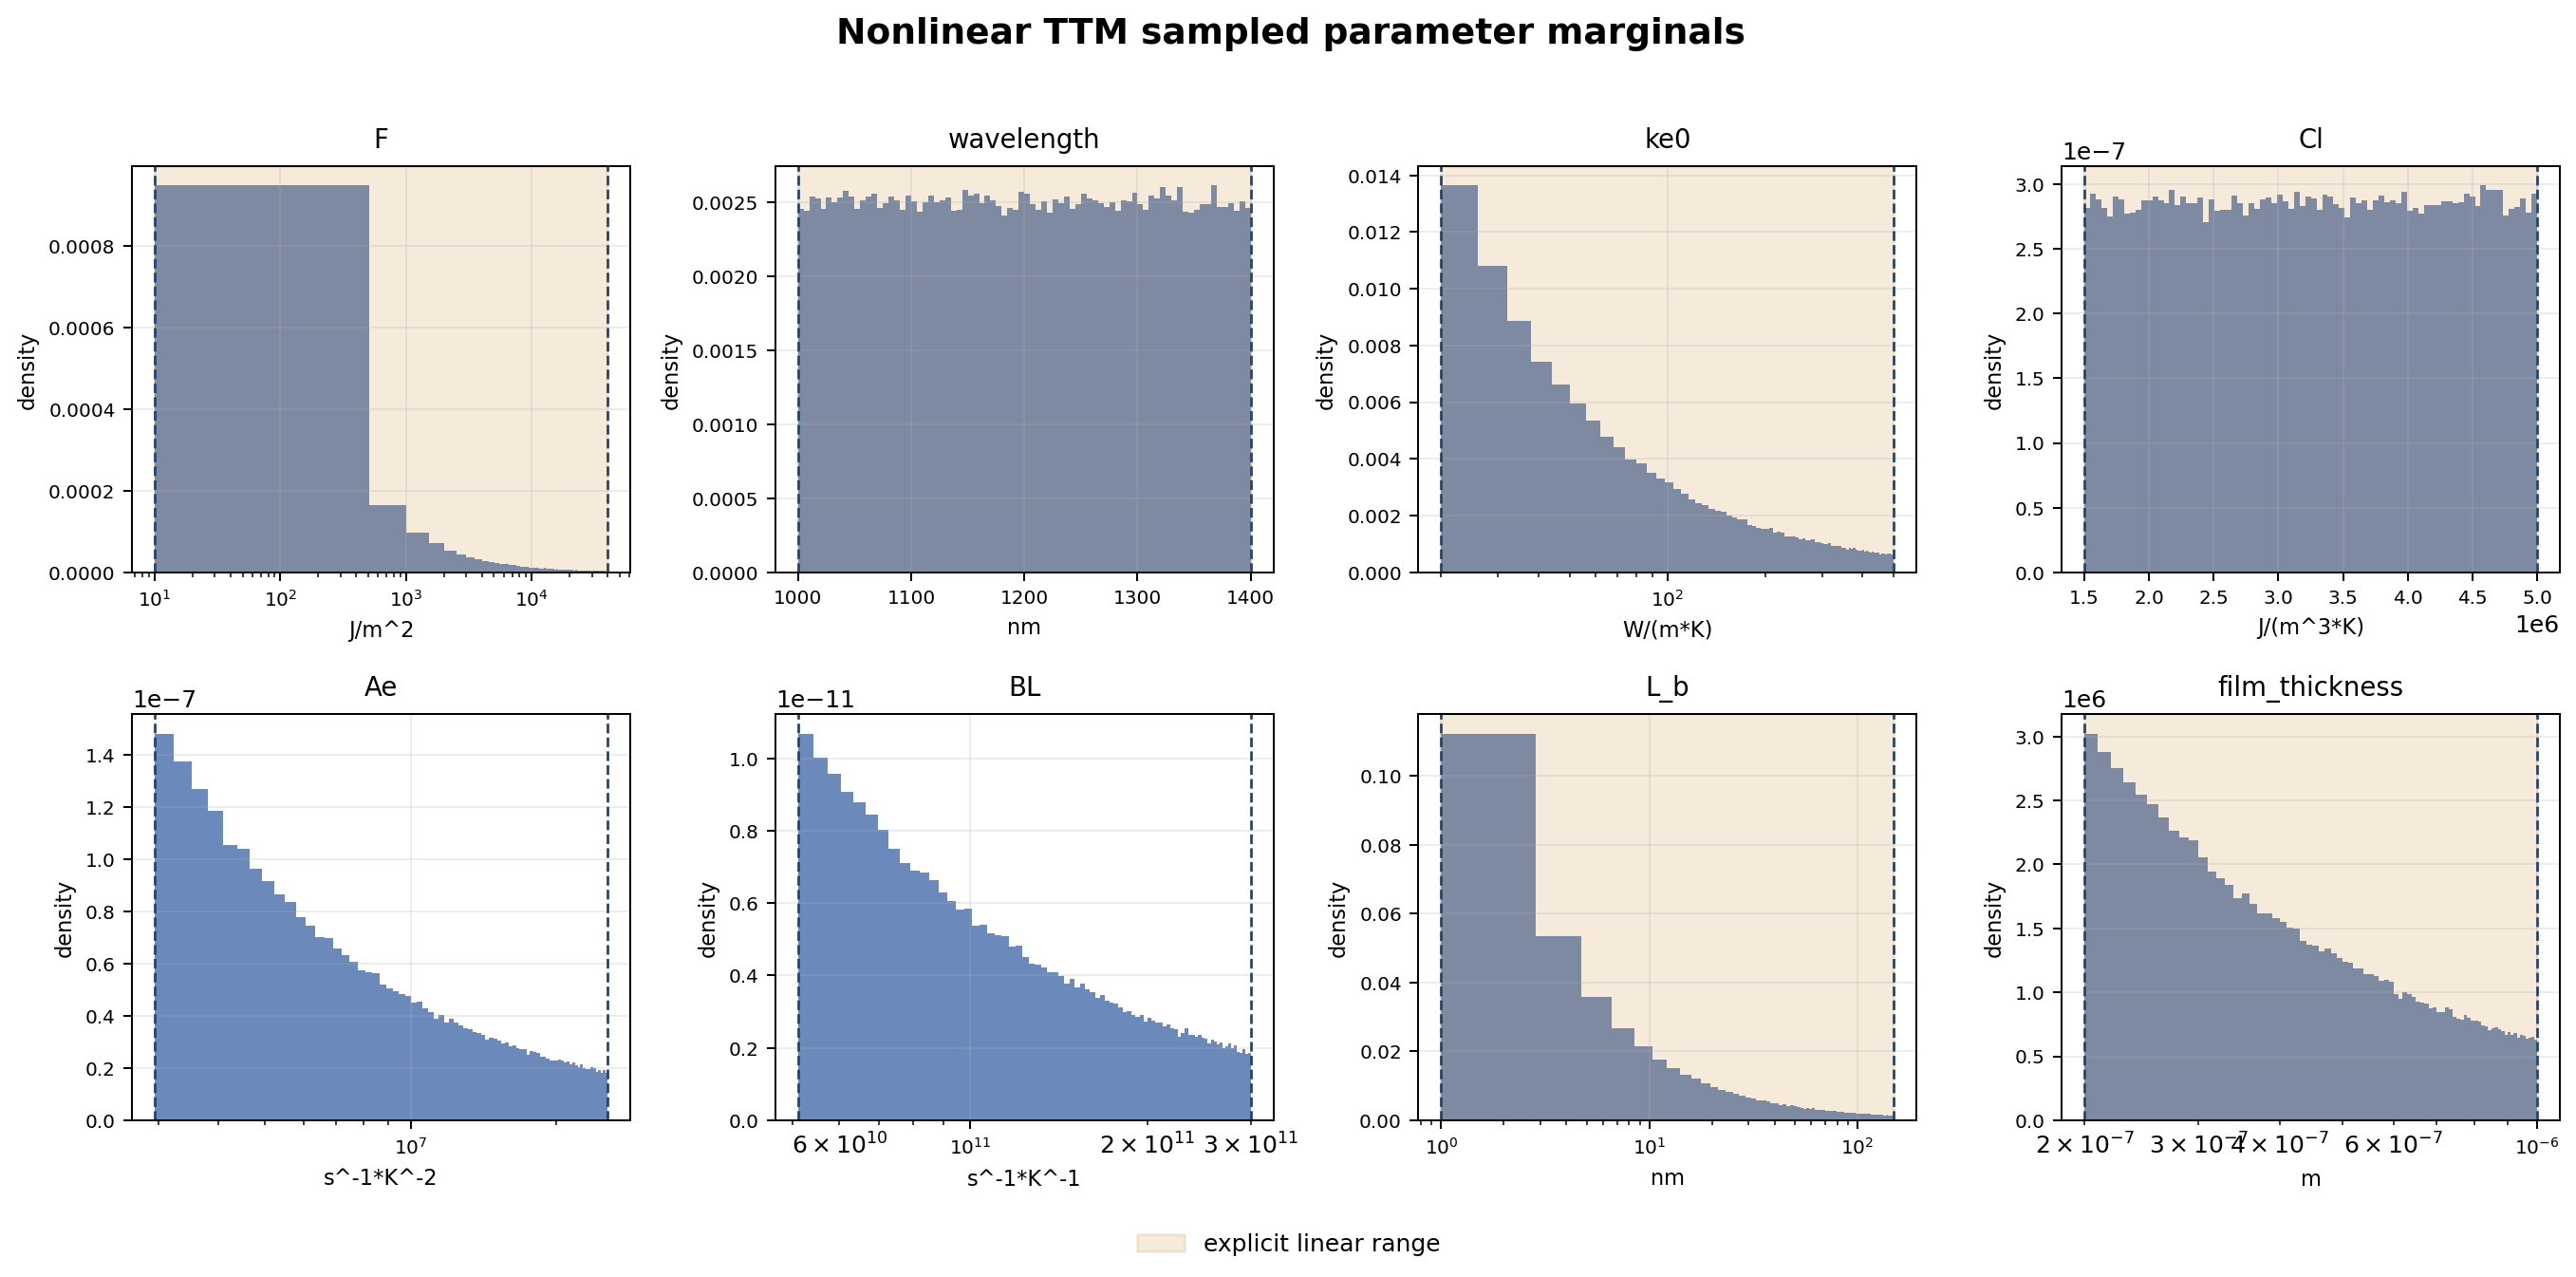
\includegraphics[width=0.96\textwidth]{figures/ch4/nonlinear_ttm/nonlinear_sampled_parameter_marginals.png}
    \caption{Marginal distributions of sampled nonlinear scalar and Lorentz--Drude descriptor inputs before deriving optical source quantities.}
    \label{fig:app-ch4-nonlinear-sampled-marginals}
\end{figure}

\begin{figure}[H]
    \centering
    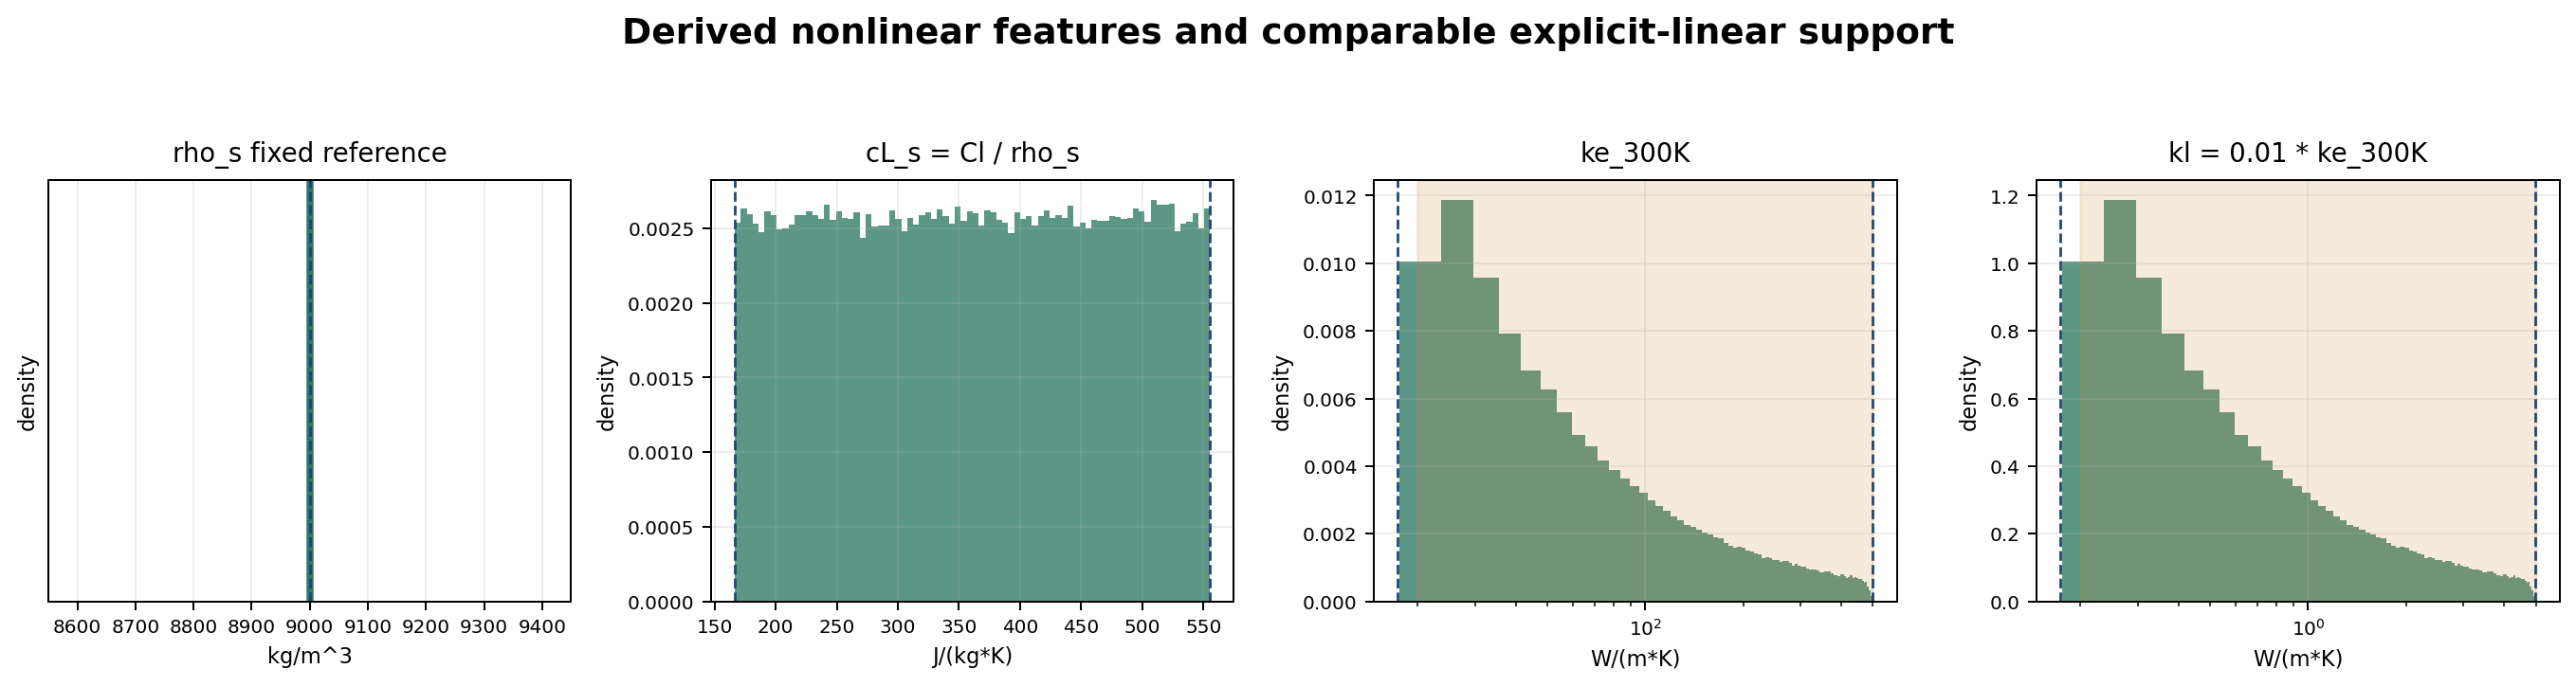
\includegraphics[width=0.96\textwidth]{figures/ch4/nonlinear_ttm/nonlinear_derived_parameter_marginals.png}
    \caption{Marginal distributions of derived nonlinear quantities, including optical source quantities obtained from sampled Lorentz--Drude descriptors.}
    \label{fig:app-ch4-nonlinear-derived-marginals}
\end{figure}

\begin{figure}[H]
    \centering
    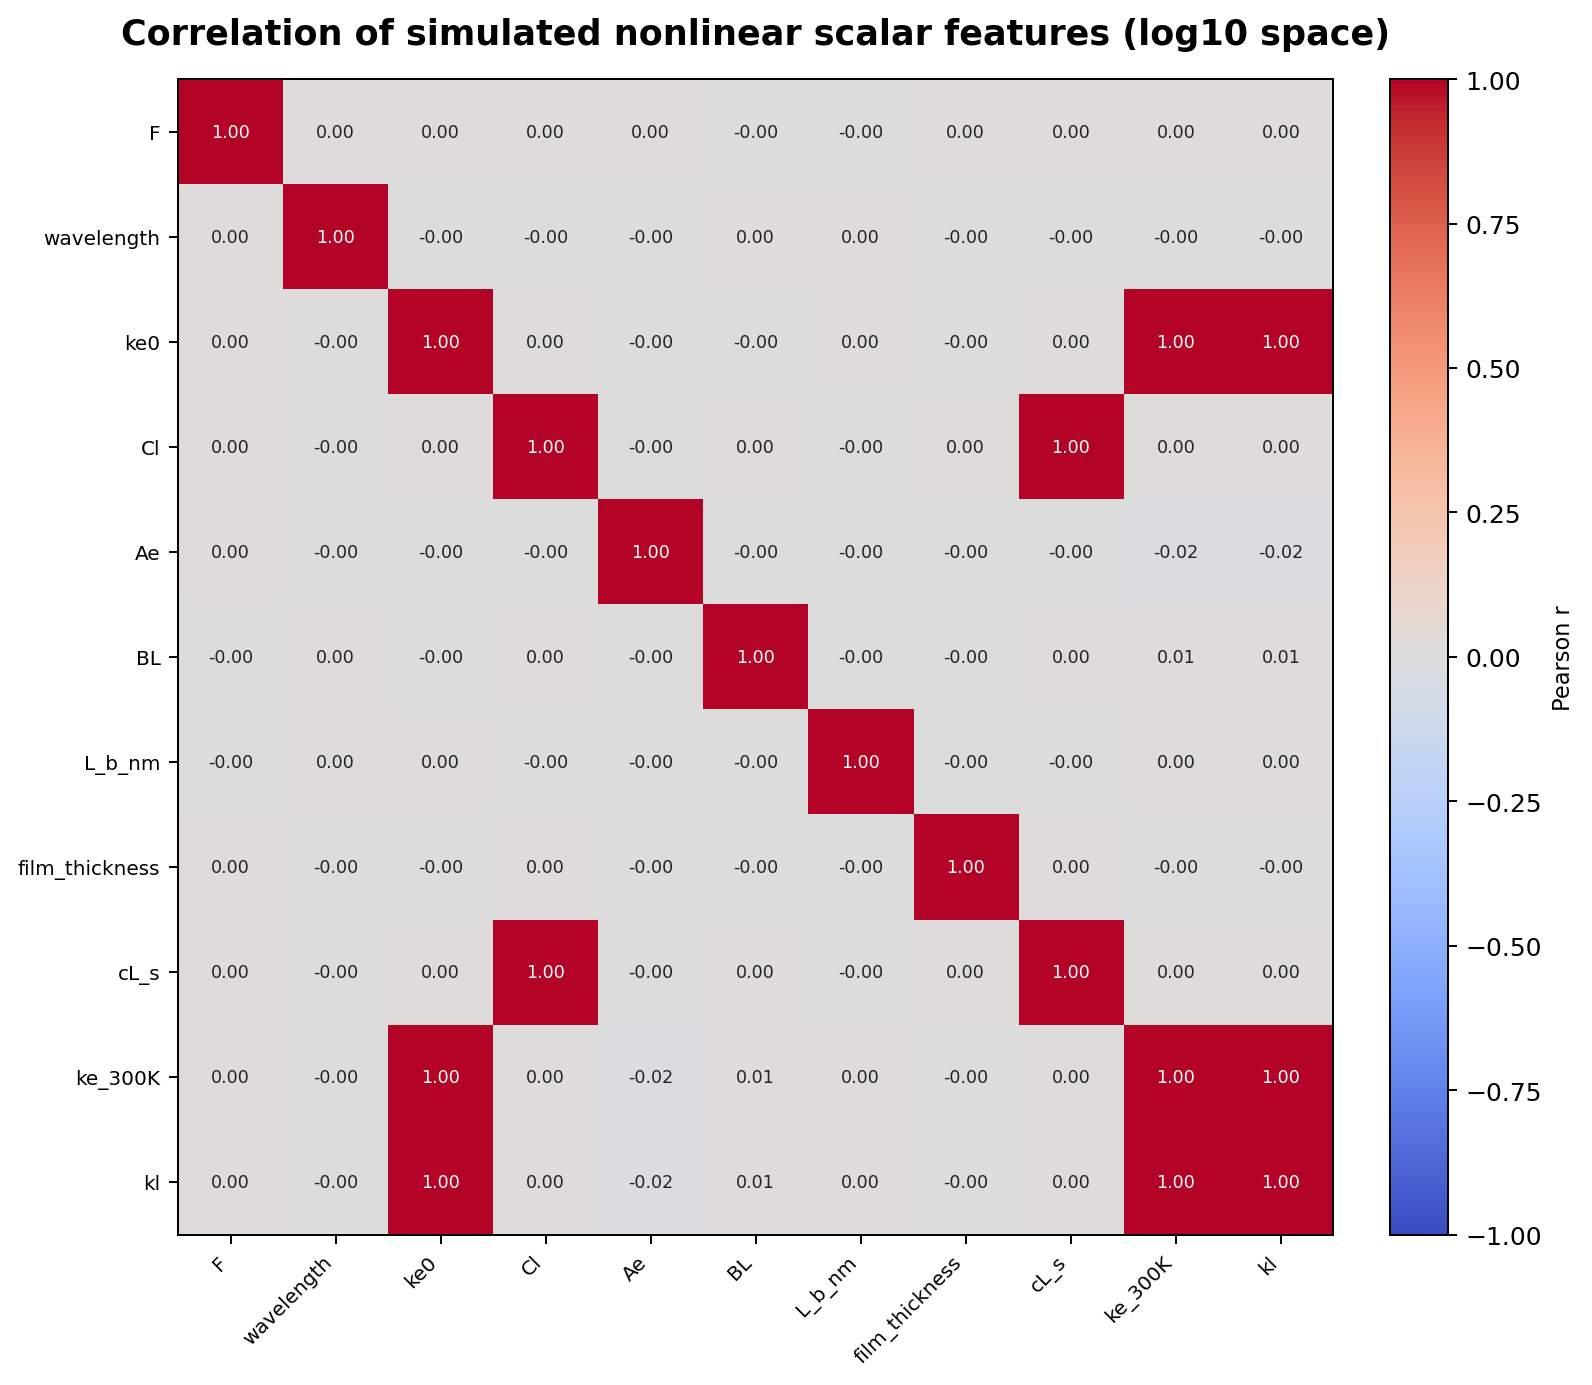
\includegraphics[width=0.82\textwidth]{figures/ch4/nonlinear_ttm/nonlinear_scalar_feature_correlation.png}
    \caption{Correlation structure among nonlinear scalar and derived features induced by the descriptor-to-source transformation.}
    \label{fig:app-ch4-nonlinear-correlation-diagnostic}
\end{figure}

\section{Nonlinear 2D TTM generation and acceptance diagnostics}

The staged nonlinear dataset used the production grid and accepted-sample policy summarised in Table~\ref{tab:appc-nonlinear-stage-20k-generation}. The table records generation and acceptance diagnostics only; it is included to document the computational provenance of the nonlinear surrogate inputs.

\begin{table}[H]
    \centering
    \caption{Generation and acceptance diagnostics for the staged 20,000-sample nonlinear 2D TTM dataset.}
    \label{tab:appc-nonlinear-stage-20k-generation}
    \small
    \begin{tabular}{p{0.32\textwidth}p{0.56\textwidth}}
\toprule
Quantity & Value \\
\midrule
Run identifier & \texttt{nonlinear\_pm1\_c4\_tail\_modal\_stage\_20k} \\
Grid & $N_x=101$, $N_z=101$, $N_t=201$ \\
Backend & CPU with PyPardiso sparse solves \\
GPU requested/effective & False / False \\
Sampler & Fixed log-spline coefficients with $\pm 1$ envelope and $c_4$ tail constraint \\
Requested shards & 200 \\
Completed shards & 200 \\
Accepted samples & 20000 \\
Attempts & 22153 \\
Rejected or diverged samples & 2153 \\
Acceptance rate & $90.2812\%$ \\
Rejection reason & Solver diverged or incomplete after accepted-sample cleaning \\
Manifest span & 32.70 h \\
Accepted samples per hour & 611.6 \\
Successful manifest container-hours & 200.508 \\
Runtime per accepted sample & p50 39.02 s; p90 43.13 s; p95 43.72 s \\
Observed preemptions & At least 14 \\
\bottomrule
\end{tabular}

\end{table}

\section{Source-term-informed feature set}

The nonlinear surrogate used the source-term-informed feature set. The internal analysis identifier was \texttt{source\_enhanced}; this identifier is retained only for reproducibility. Table~\ref{tab:appc-nonlinear-selected-features} gives the compact definition of the feature groups, including the source-prefactor descriptors. The product $F\chi_{S,0}$ is a prefactor descriptor for the laser source, not the complete volumetric source term.

\begin{table}[H]
    \centering
    \caption{Compact definition of the source-term-informed feature set used in the nonlinear surrogate analysis.}
    \label{tab:appc-nonlinear-selected-features}
    \scriptsize
    \begin{tabular}{p{0.22\textwidth}p{0.22\textwidth}p{0.46\textwidth}}
\toprule
Feature group & Included descriptors & Definition or role \\
\midrule
\multicolumn{3}{p{0.92\textwidth}}{Feature set name used in the thesis: source-term-informed feature set. Internal analysis identifier: \texttt{source\_enhanced}.} \\
\midrule
Sampled scalar inputs & $F$, $k_{e0}$, $C_l$, $A_e$, $B_L$, $L_b$, $h$, $\lambda$ & Incident fluence, conductivity scale, lattice heat capacity, conductivity-model coefficients, ballistic length, film thickness, and wavelength. \\
Derived optical inputs & $\alpha$, $R$ & Absorption coefficient and reflectivity derived from the Lorentz--Drude optical descriptor sample at the reference state. \\
Room-temperature curve summaries & $C_e(T_0)$, $G(T_0)$ & Values of the nonlinear thermophysical curves at $T_0=\SI{300}{\kelvin}$. \\
Grid curve summaries & $C_{e,\min}^{\mathcal{T}}$, $C_{e,\max}^{\mathcal{T}}$, $G_{\min}^{\mathcal{T}}$, $G_{\max}^{\mathcal{T}}$ & Minimum and maximum values over the accepted thermophysical evaluation grid $\mathcal{T}$, spanning \SI{300}{\kelvin} to \SI{50000}{\kelvin}. \\
Log-spline coefficients & $c^{C_e}_0,\ldots,c^{C_e}_6$ and $c^G_0,\ldots,c^G_6$ & Cubic B-spline coefficients for $\log C_e(T_e)$ and $\log G(T_e)$, with the high-temperature tail constraint $c_5=c_4$ and $c_6=c_4$ for each property. \\
Ballistic-corrected absorption & $\alpha_{\mathrm{eff},0}$ & $\alpha_{\mathrm{eff},0}=\alpha_0/(1+\alpha_0 L_b)$, using $L_b$ in metres. \\
Source prefactor & $\chi_{S,0}$ & $\chi_{S,0}=\alpha_{\mathrm{eff},0}(1-R_0)/(1-\exp(-\alpha_{\mathrm{eff},0}h))$. \\
Fluence-source interaction & $F\chi_{S,0}$ & Product of incident fluence and source prefactor. This is a source-prefactor descriptor, not the full volumetric source term. \\
\bottomrule
\end{tabular}

\end{table}

\begin{figure}[H]
    \centering
    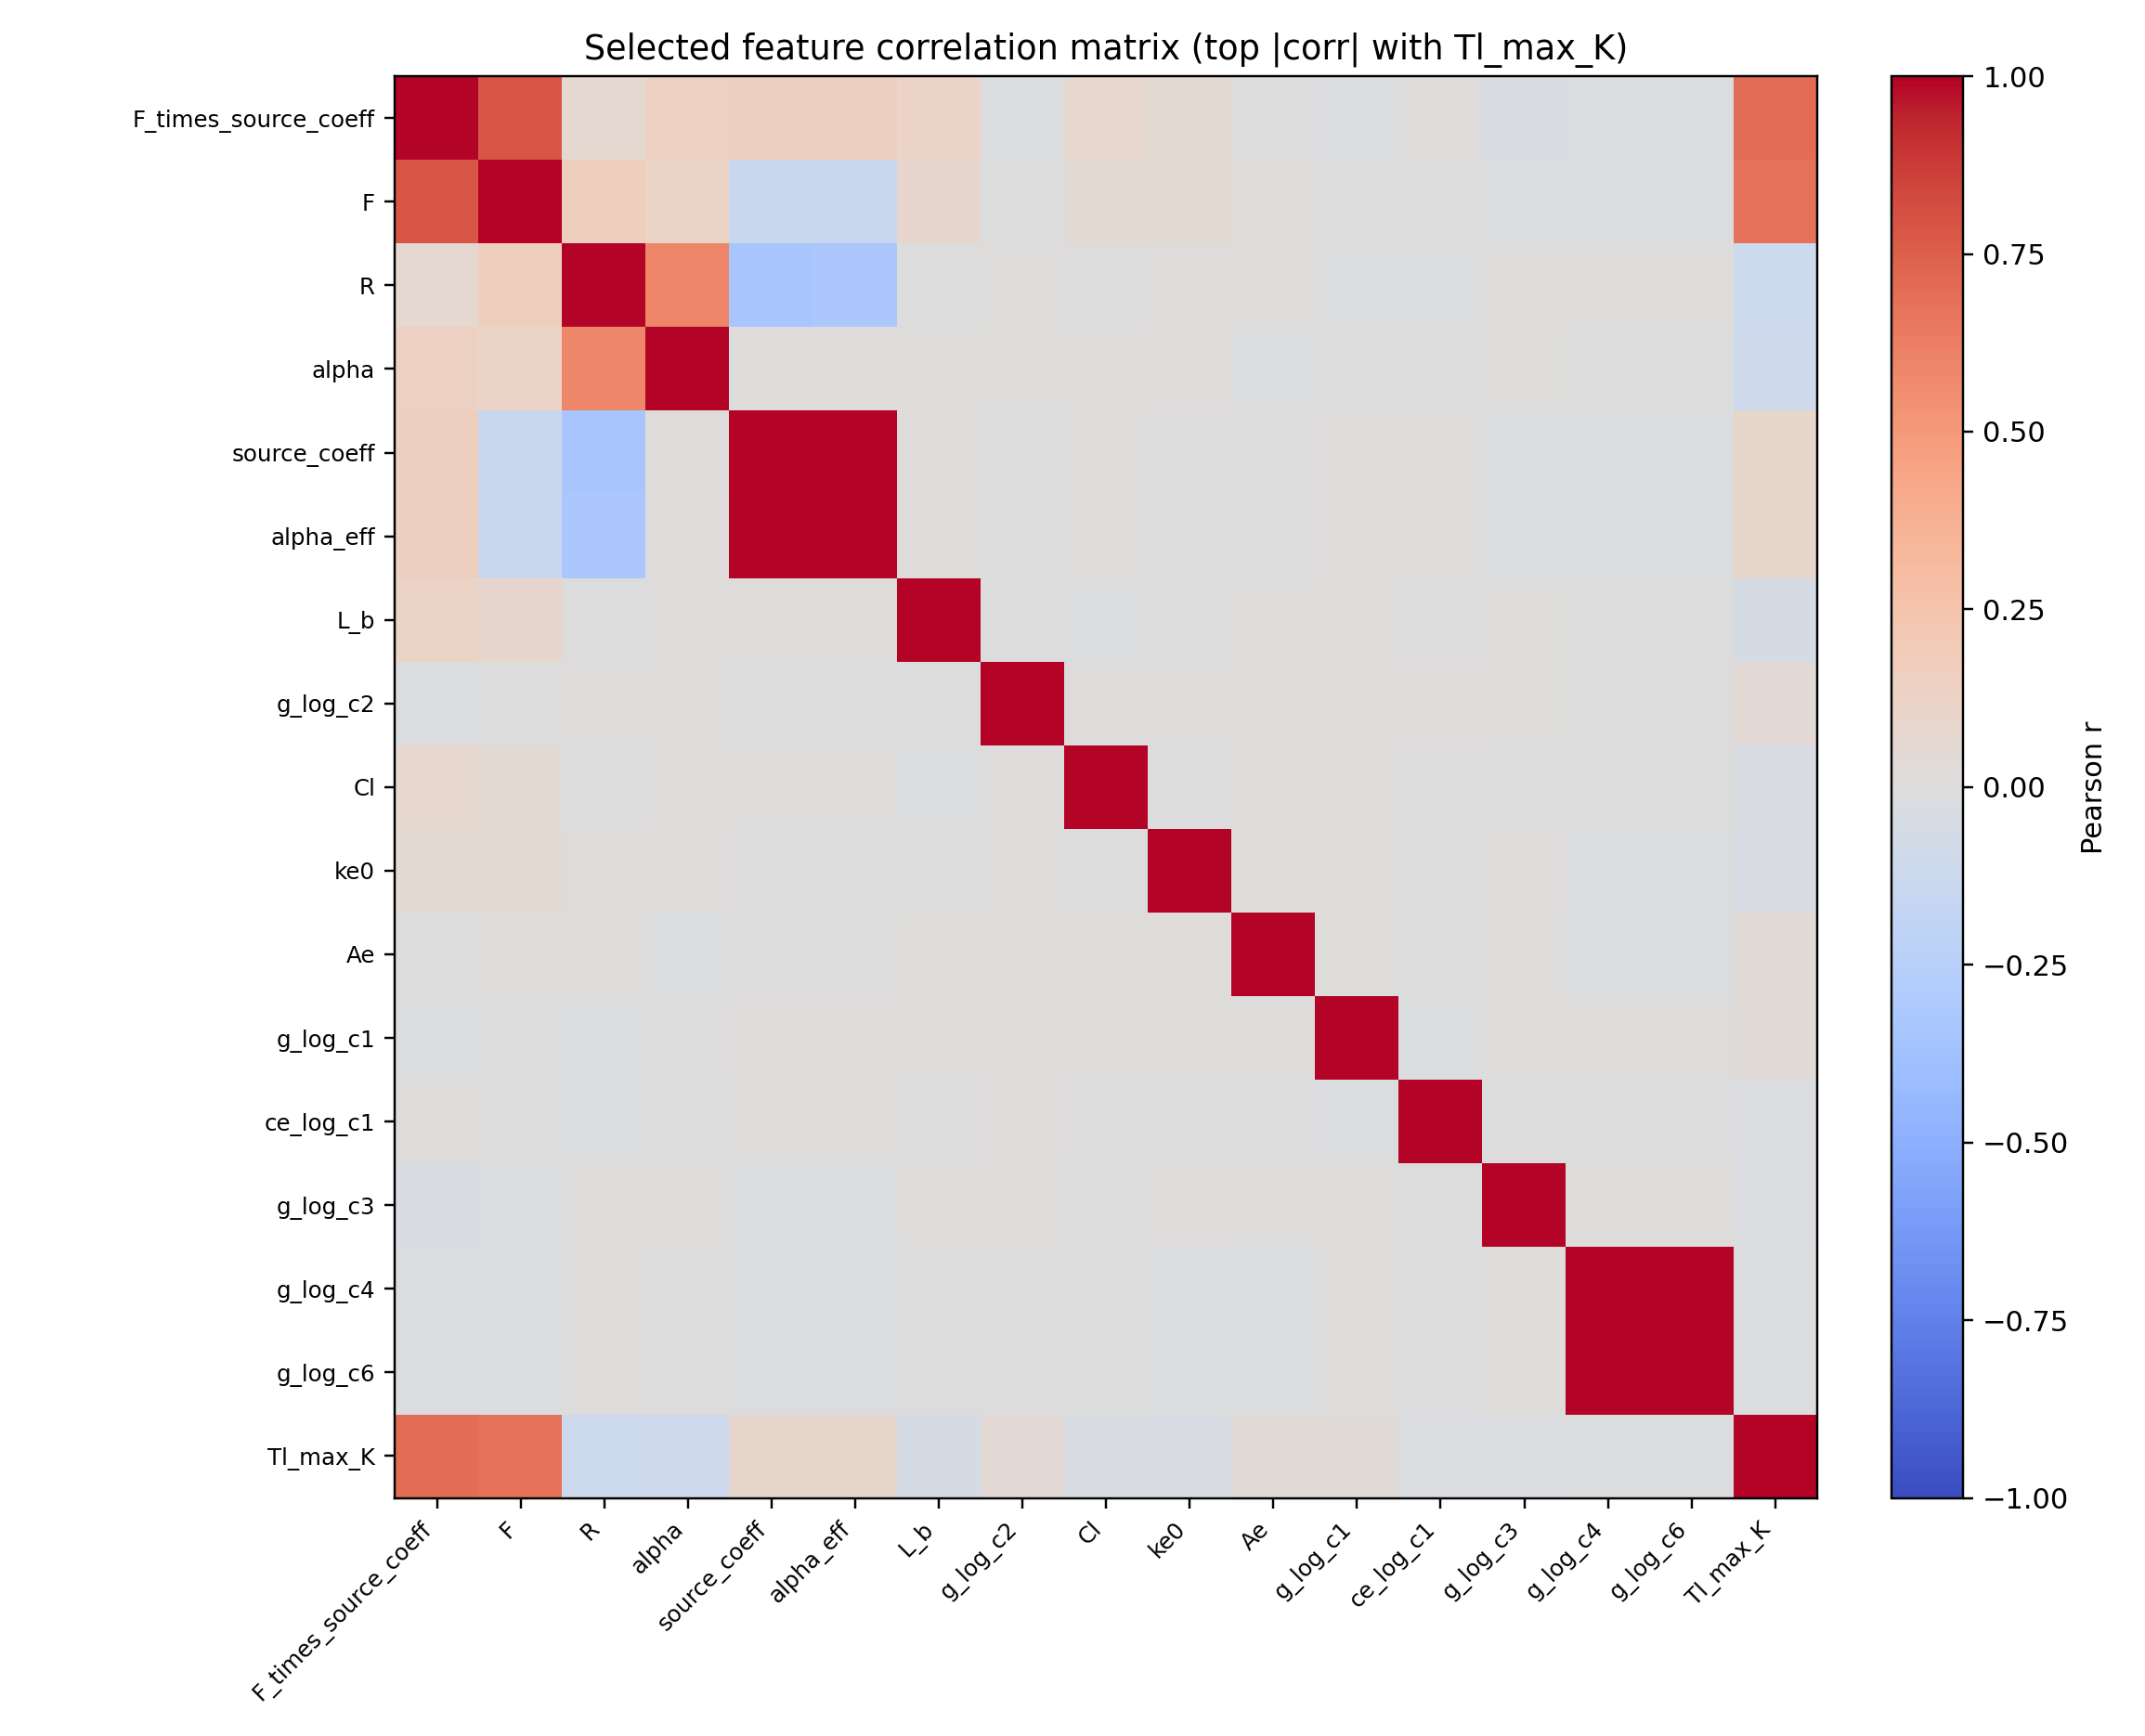
\includegraphics[width=0.96\textwidth]{figures/ch4/nonlinear_ttm/final_20k/selected_feature_correlation_matrix.png}
    \caption{Correlation matrix for the selected source-term-informed nonlinear feature set. The dense matrix is retained as an appendix diagnostic rather than a main-text figure.}
    \label{fig:appc-nonlinear-selected-feature-correlation}
\end{figure}

\section{Nonlinear model configurations}

The held-out nonlinear surrogate metrics are reported in Table~\ref{tab:ch4-nonlinear-model-metrics}. Table~\ref{tab:appc-nonlinear-model-configurations} documents the fixed bounded configurations used for the 20,000-sample nonlinear analysis. A full nonlinear hyperparameter optimisation was not run for this dataset.

\begin{table}[H]
    \centering
    \caption{Model configurations used in the nonlinear 2D TTM surrogate analysis.}
    \label{tab:appc-nonlinear-model-configurations}
    \scriptsize
    \begin{tabular}{p{0.13\textwidth}p{0.17\textwidth}p{0.39\textwidth}p{0.11\textwidth}}
\toprule
Model & Preprocessing & Configuration & HPO status \\
\midrule
LightGBM & Native tabular inputs & \texttt{gbdt}; 500 estimators; learning rate 0.04; 63 leaves; subsample 0.9; column subsample 0.9; $L_1=0.001$; $L_2=0.01$; random state 42; single job. & Fixed bounded \\
MLP & StandardScaler & scikit-learn MLPRegressor; hidden layers $(128,64)$; $\alpha=10^{-4}$; batch size 256; learning rate 0.001; max iterations 350; early stopping; random state 42. & Fixed bounded \\
\bottomrule
\end{tabular}

\end{table}

\section{Nonlinear material-validation diagnostics}

Table~\ref{tab:appc-nonlinear-material-availability} records which real-material nonlinear validation cases were available. Table~\ref{tab:appc-nonlinear-material-metrics} then summarises the material-validation metrics for those available cases. Figures~\ref{fig:appc-nonlinear-ag-validation}--\ref{fig:appc-nonlinear-cu-validation} give the supplementary noble-metal validation overlays.

\begin{table}[H]
    \centering
    \caption{Material availability for the nonlinear validation and threshold checks.}
    \label{tab:appc-nonlinear-material-availability}
    \small
    \begin{tabular}{lccp{0.47\textwidth}}
\toprule
Material & Nonlinear curves & Direct curve & Note \\
\midrule
Ag & Yes & Yes & Nonlinear $C_e/G$ curves and optical entries available. \\
Au & Yes & Yes & Nonlinear $C_e/G$ curves and optical entries available. \\
Cu & Yes & Yes & Nonlinear $C_e/G$ curves and optical entries available. \\
Ni & Yes & Yes & Nonlinear $C_e/G$ curves and optical entries available. \\
Ti & Yes & Yes & Nonlinear $C_e/G$ curves and optical entries available. \\
Cr & No & No & Missing material-specific nonlinear $C_e/G$ curves. \\
Al & No & No & Missing material-specific nonlinear $C_e/G$ curves. \\
\bottomrule
\end{tabular}

\end{table}

\begin{table}[H]
    \centering
    \caption{Material-validation metrics for available nonlinear real-material curves.}
    \label{tab:appc-nonlinear-material-metrics}
    \small
    \begin{tabular}{llrrrr}
\toprule
Material & Model & Points & RMSE (K) & MAE (K) & $R^2$ \\
\midrule
Ag & LightGBM & 15 & 354.943 & 135.266 & 0.438 \\
Ag & MLP & 15 & 268.714 & 89.939 & 0.678 \\
Au & LightGBM & 15 & 1693.643 & 515.535 & 0.269 \\
Au & MLP & 15 & 1765.201 & 587.993 & 0.206 \\
Cu & LightGBM & 15 & 769.851 & 229.272 & 0.434 \\
Cu & MLP & 15 & 796.774 & 288.212 & 0.394 \\
Ni & LightGBM & 13 & 234.346 & 109.586 & 0.986 \\
Ni & MLP & 13 & 217.462 & 152.604 & 0.988 \\
Ti & LightGBM & 11 & 169.601 & 113.626 & 0.993 \\
Ti & MLP & 11 & 309.705 & 166.363 & 0.976 \\
\bottomrule
\end{tabular}

\end{table}

\begin{figure}[H]
    \centering
    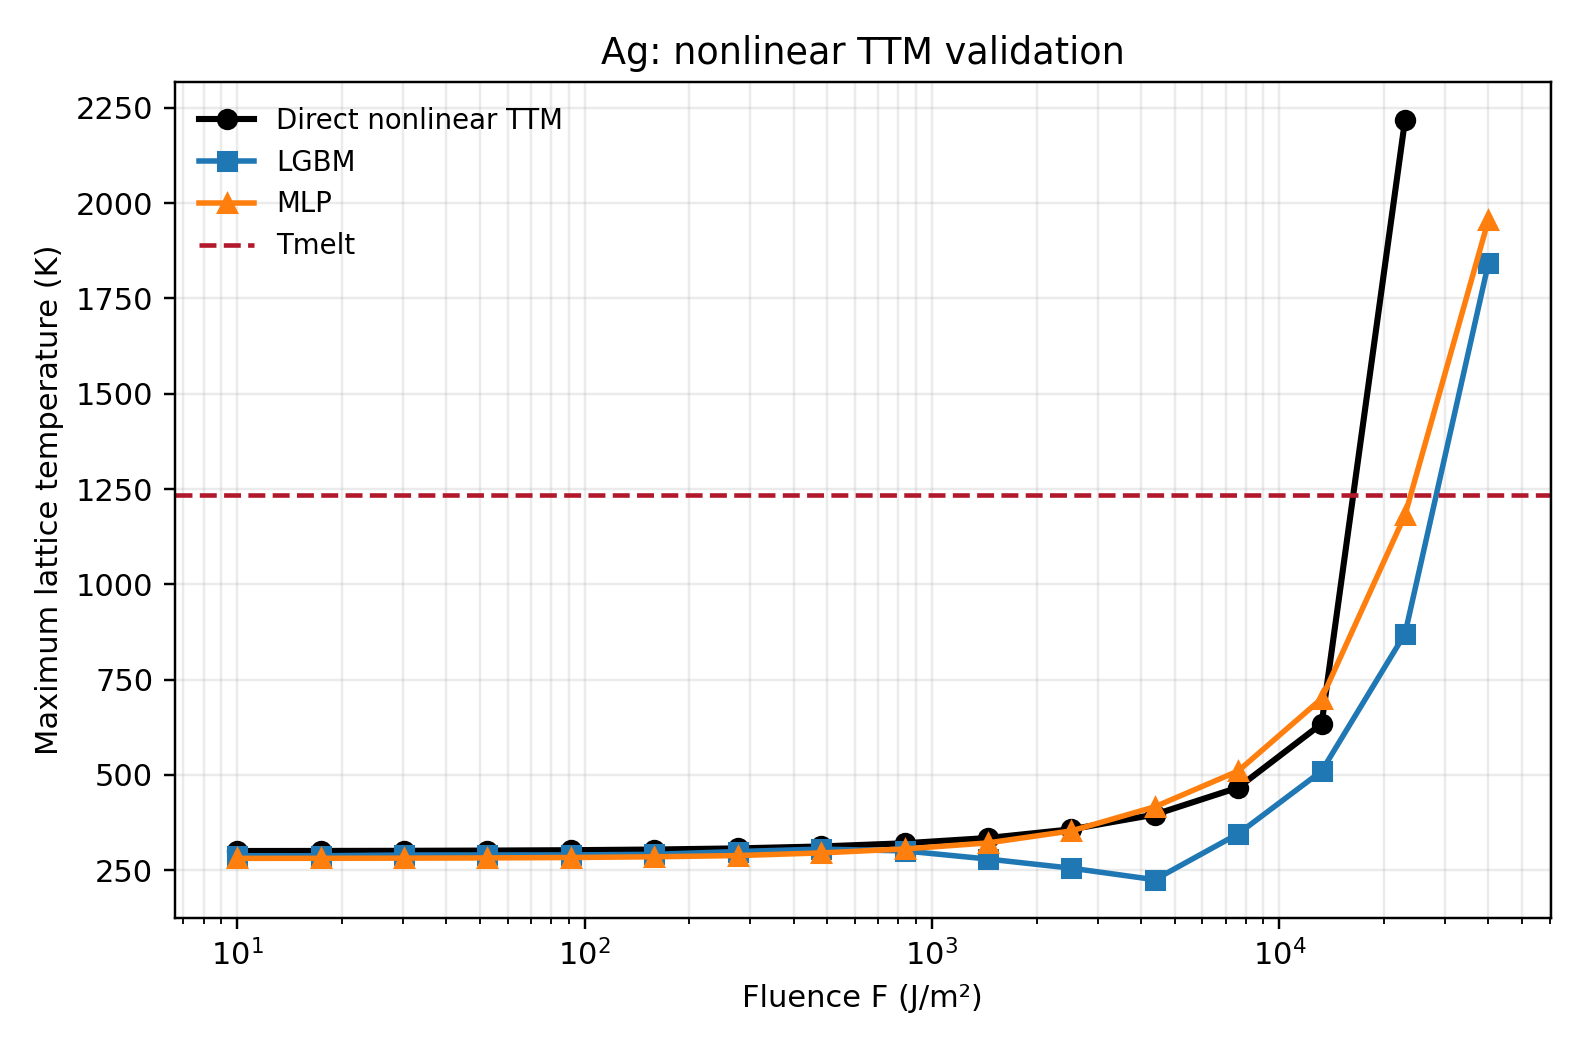
\includegraphics[width=0.78\textwidth]{figures/ch4/nonlinear_ttm/final_20k/nonlinear_Ag_validation.png}
    \caption{Ag nonlinear material-validation overlay for the source-term-informed LightGBM and MLP surrogates.}
    \label{fig:appc-nonlinear-ag-validation}
\end{figure}

\begin{figure}[H]
    \centering
    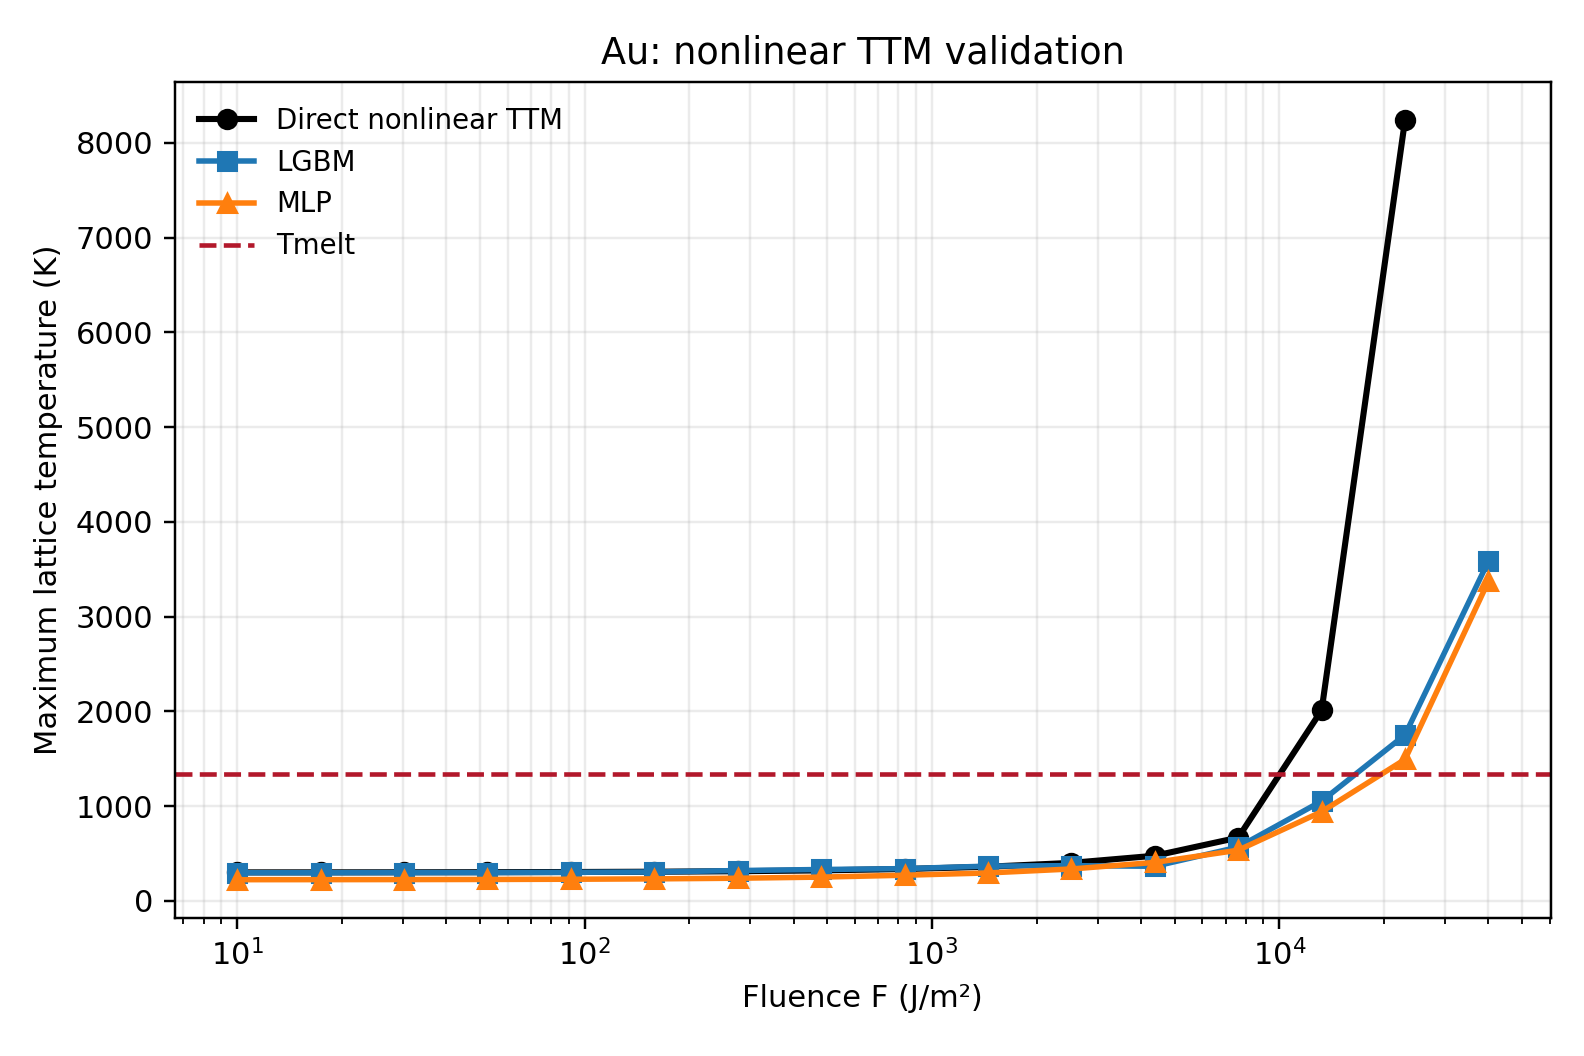
\includegraphics[width=0.78\textwidth]{figures/ch4/nonlinear_ttm/final_20k/nonlinear_Au_validation.png}
    \caption{Au nonlinear material-validation overlay for the source-term-informed LightGBM and MLP surrogates.}
    \label{fig:appc-nonlinear-au-validation}
\end{figure}

\begin{figure}[H]
    \centering
    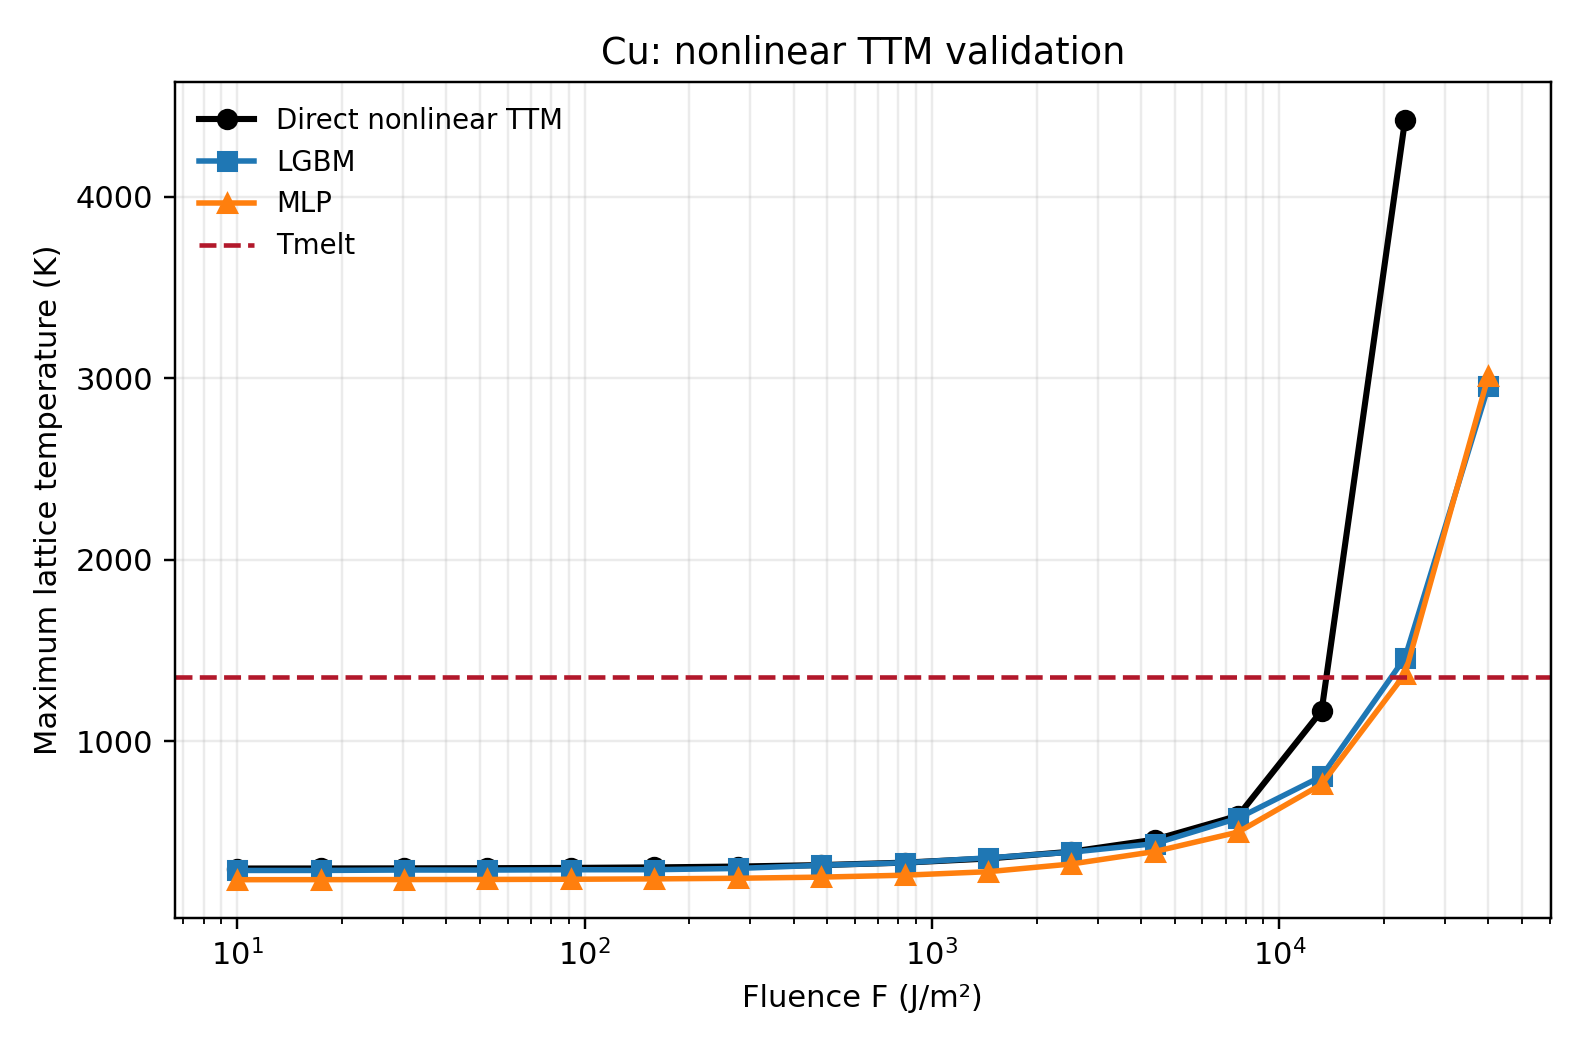
\includegraphics[width=0.78\textwidth]{figures/ch4/nonlinear_ttm/final_20k/nonlinear_Cu_validation.png}
    \caption{Cu nonlinear material-validation overlay for the source-term-informed LightGBM and MLP surrogates.}
    \label{fig:appc-nonlinear-cu-validation}
\end{figure}

\section{External threshold comparisons}

External cross-model threshold values and the corresponding comparison graphics are omitted from this public source pending documented redistribution terms.

\section{Grid-refinement check for direct nonlinear thresholds}

The grid-refinement diagnostics below report only internally generated direct nonlinear threshold calculations.

\begin{figure}[H]
    \centering
    \subfloat[Direct nonlinear threshold stability on the refined grid for available material cases.\label{fig:appc-nonlinear-high-grid-stability}]{%
        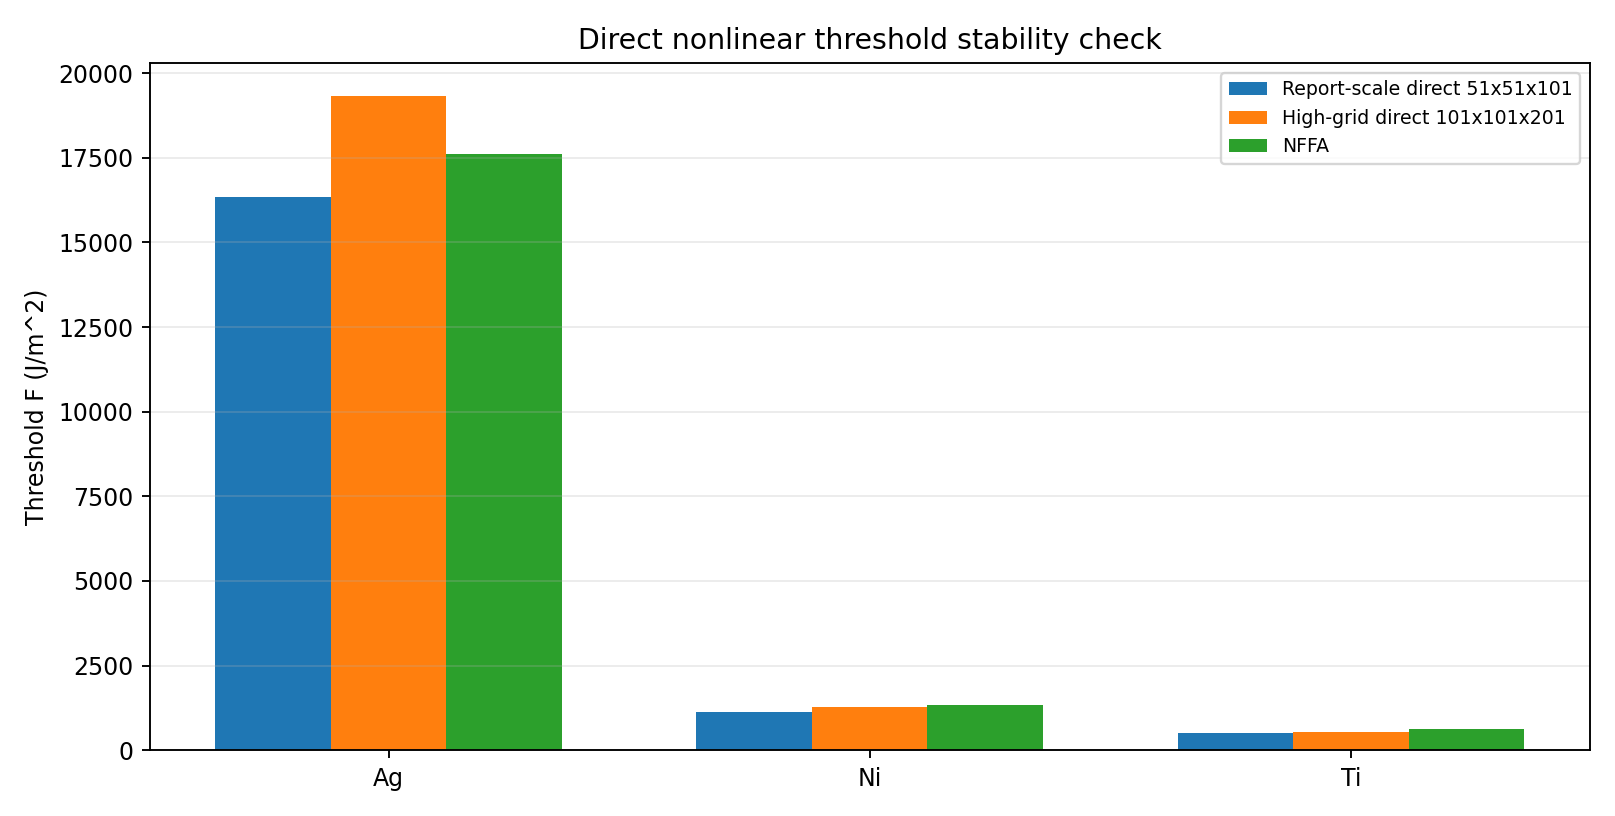
\includegraphics[width=0.48\textwidth]{figures/ch4/nonlinear_ttm/final_20k/high_grid_threshold_stability.png}
    }
    \hfill
    \subfloat[Relative change between report-grid and refined-grid direct nonlinear thresholds.\label{fig:appc-nonlinear-high-grid-delta}]{%
        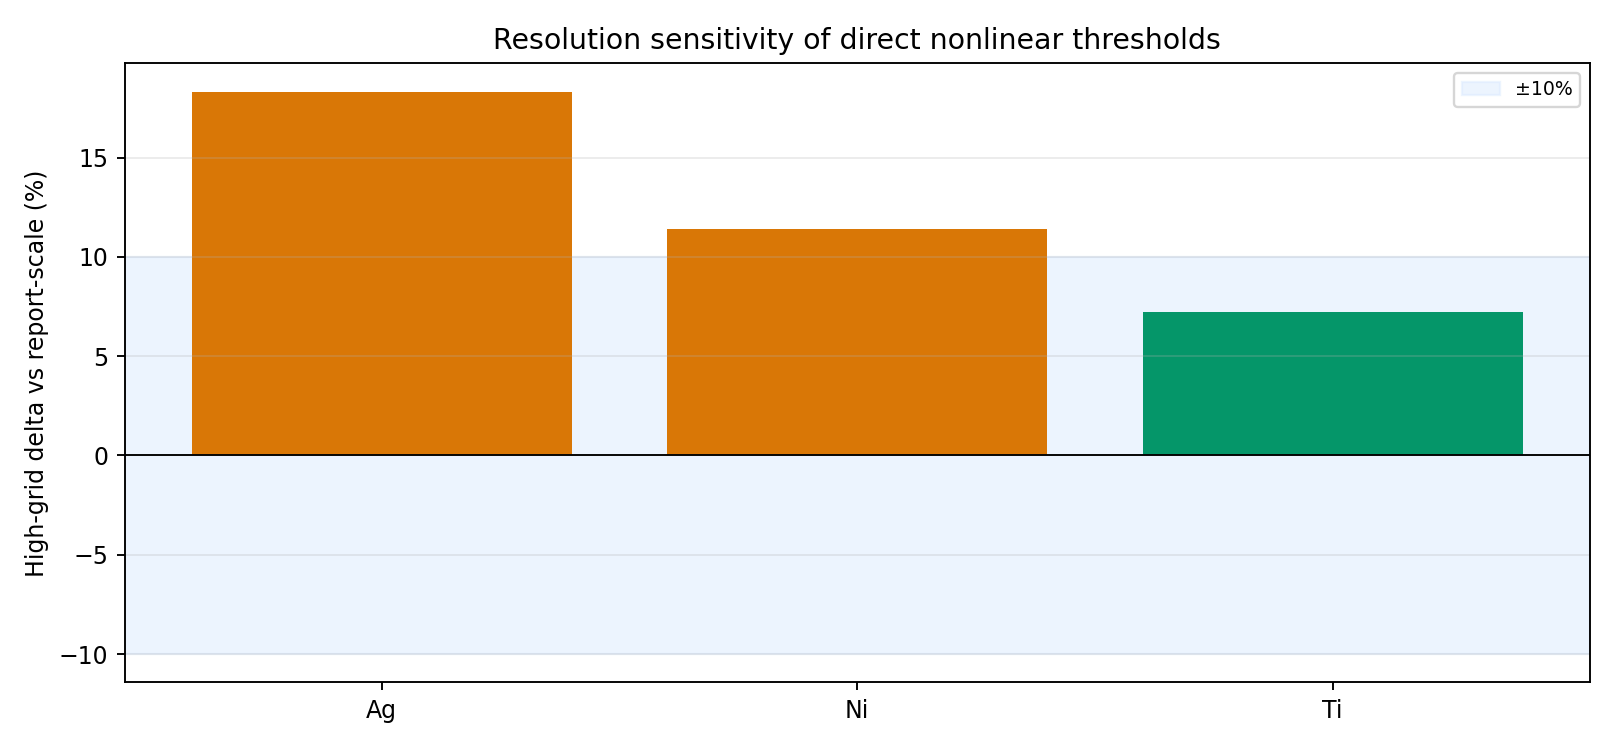
\includegraphics[width=0.48\textwidth]{figures/ch4/nonlinear_ttm/final_20k/high_grid_delta_vs_report.png}
    }
    \caption{Grid-refinement diagnostics for the direct nonlinear Ag, Ni, and Ti threshold checks.}
    \label{fig:appc-nonlinear-high-grid-summary}
\end{figure}
